\documentclass[10pt,conference,draftclsnofoot,onecolumn]{IEEEtran}
\usepackage{listings}
\usepackage[dvipsnames]{xcolor}
\usepackage{color}
\usepackage{anysize}
\usepackage{hyperref}
\usepackage[backend=bibtex]{biblatex}
\usepackage{amsmath}
\marginsize{2cm}{2cm}{2cm}{2cm}
\addbibresource{bib.bib}

\lstdefinelanguage
   [x86Extended]{Assembler}     % add an "x86Extended dialect of Assembler
   [x86masm]{Assembler}         % based on the "x86masm" dialect
   % Define new keywords
   {morekeywords={rdrand, cpuid}}

\lstdefinestyle{customc}{
  belowcaptionskip=1\baselineskip,
  breaklines=true,
  frame=L,
  xleftmargin=\parindent,
  language=C,
  showstringspaces=false,
  basicstyle=\footnotesize\ttfamily,
  keywordstyle=\bfseries\color{OliveGreen},
  commentstyle=\itshape\color{Fuchsia},
  identifierstyle=\color{black},
  stringstyle=\color{Bittersweet},
}

\lstdefinestyle{customasm}{
  belowcaptionskip=1\baselineskip,
  frame=L,
  xleftmargin=\parindent,
  language=[x86masm]Assembler,
  basicstyle=\footnotesize\ttfamily,
  commentstyle=\itshape\color{Fuchsia},
}

\lstset{escapechar=@,style=customc}

\usepackage{graphicx}

\begin{document}

\begin{titlepage}
\author{\IEEEauthorblockN{Ian Kronquist}
\IEEEauthorblockA{School of Electrical and\\Computer Science\\
Oregon State University\\
Corvallis, Oregon\\
kronquii@oregonstate.edu}
\and
\IEEEauthorblockN{Sempon ``Sibi'' Kabilan}
\IEEEauthorblockA{School of Electrical and\\Computer Science\\
Oregon State University\\
Corvallis, Oregon\\
kabilans@oregonstate.edu}
\and
\IEEEauthorblockN{Zach Torres}
\IEEEauthorblockA{School of Electrical and\\Computer Science\\
Oregon State University\\
Corvallis, Oregon\\
torresz@oregonstate.edu}
}

\title { Next Generation Open Source Honeypot: \\Spring 2016 Midterm Report}
\maketitle
    \centering
    {\Large Oregon State University Senior Capstone Project\\ \par}
    {\Large Team 13\\\par}
    \vspace{1.5cm}



    \begin{abstract}
    Security researchers are in a constant race to catch the latest kinds of malware to secure the public. To catch new kinds of malware they use honeypots, which are computers being monitored by researchers and running vulnerable software so they will be purposefully infected by malware. State of the art honeypots for the WordPress blogging platform do not catch the newest varieties of malware. For our senior project we wrote an open source honeypot which can detect attacks from common WordPress malware. Our honeypot uses a novel design to leverage new Linux Kernel based technologies like Docker to securely contain and observe malware.

    \end{abstract}
    \vfill
% Bottom of the page
    {\large \today\par}


\end{titlepage}

\section{Introduction}
Malware researchers use virtual traps called honeypots to gather information about new techniques malware use to gain access to sensitive systems. These honeypots are deployed to mimic vulnerable servers or systems that are targets for malware in a safe environment. While some honeypots are designed to capture malware samples, there are also those that are designed to prevent intrusions and even counteract against attacks. The honeypots that capture malware samples and secure said samples before sending them to centralized repositories that collect malware samples for later analysis called honeyfeeds. This task is vital for the cyber security industry as it keeps them apprised of developments in malware and other attacks. It also provides information regarding commonly exploited vulnerabilities in widely used software. This information is then used to produce fixes for the software and close identified vulnerabilities. However, most of the current honeypots are outdated and are in dire need of updates. They lack the ability to mimic the targets that are currently trending, such as the WordPress blogging platform. This gap arises due to the fact that most malware was designed for a previous generation of servers and software stacks. Even the ones currently updated and maintained regularly are designed for server level architecture. This results in honeypots that are more concentrated in preventing and counteracting attacks than collecting malware samples. The older generation sample collection honeypots are less than ideal in collecting newer and trending malware samples, sometimes even completely missing out on samples from entire platforms. 

\section{Project Problem}
Security researchers are in a constant race with hackers to find the latest kinds of malware and secure our computers. To find new kinds of malware, researchers use honeypots which are special computers under observation which run vulnerable software.

WordPress is an open source blogging platform written in PHP which is notorious for its vulnerabilities. Hackers will often attack WordPress blogs and then use those sites to pivot and attack other hosts in the same network, or use those hosts to perform Distributed Denial of Service or other attacks. Other honeypots exist to monitor WordPress website, most notably WordPot. Unfortunately, WordPot doesn’t find the latest types of WordPress malware and it is easy for malware to detect that it is actually interacting with a honeypot. One of the most common vectors for infecting WordPress websites are third party plugins which add additional functionality. Unfortunately, WordPot cannot support WordPress plugins.

In order to share their  findings, many security researchers use the Modern Honeypot Network or MHN. Fleets of honeypots can report attacks to MHN for analysis. Many honeypots are run on small lightweight computers like Intel’s Minnowboard.

\section{Project Purpose}
The purpose of this project is to build a honeypot which will aid security researchers in finding the latest kinds of malware. We will write an open source honeypot capable of catching malware, detecting infection, and passing information along to the Modern Honeypot Network. The honeypot should be capable of running on resource constrained environments such as the Minnowboard.

\section{Project Goals}
The goal of the project is to be able to catch and monitor WordPress malware. In order to catch the latest kinds of malware it should be able to be easily upgraded to support newer versions of WordPress and support a variety of WordPress plugins. It should also be difficult to detect that the malware is interacting with a honeypot. It should be able to run on cheap resource constrained computers like the Intel Minnowboard so that it can be deployed widely in fleets. It should also be able to run on CentOS and Ubuntu, two of the most common free Linux distributions. The Minnowboard platform we will deploy to should be hardened to help prevent malware from escaping. Finally, our code should be robust and tested. 

Once malware infects a computer, it will frequently search for sensitive files like SSH keys, passwords, and potentially inject itself into other executables on the system. It may also send messages back to a command and control server, or start other programs. To catch malware in the act, the honeypot should be able to log any unexpected access to the file system, network traffic, or new programs which are spawned. Once malware has been detected, information about its actions should be sent to a Modern Honeypot Network server for analysis by researchers.

\section{Implementation}

\subsection{Our Architecture}
We needed to keep the malware in a secure location so it couldn’t interfere with the honeypot or otherwise attack the host system. We considered using virtual machines but decided that approach would be less flexible and may even involve patching the Linux kernel to hide our monitoring and reporting code from the malware. Fortunately Linux provides a new lighter weight solution for securely sandboxing software in the form of containers. Containers leverage network namespaces, cgroups, and other Linux specific APIs to securely isolate software. A new tool called Docker allows containers to be managed easily and securely. Docker has allowed us to make the container part of the infrastructure completely configurable so we can monitor software other than WordPress. One of our stretch goals was to modify the honeypot to monitor SSH servers, and our flexible architecture allowed us to replace WordPress with SSH with a two line configuration file change.

Our honeypot starts up several containers using a tool called Docker Compose. After the containers are started it starts three monitor processes and opens a connection to the MHN server. The monitors use Linux kernel APIs to watch for unusual activity within the container. The honeypot then passes the information gathered by the monitors through a series of filters and on to the Reporter which forwards signs of attack on to the Modern Honeypot Network.

\begin{figure}[!ht]
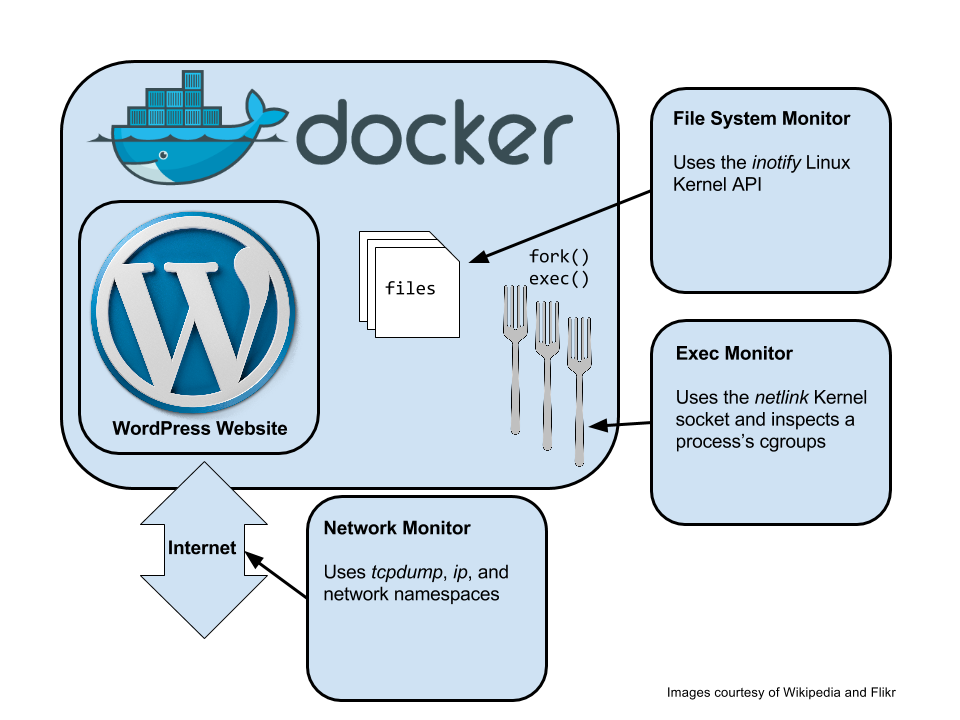
\includegraphics[scale=0.6]{./nesteddiagram.eps}
\caption{System Event Processing Pipeline}
\end{figure}



\subsection{The Pipeline}
Events which happen within the Docker containers are processed in a three stage pipeline. The first stage is the Monitor. The Monitor spawns separate child processes and reads the event information they send to standard out. It does a minimal amount of verification and passes events on to the Filter. The Filter removes unwanted events, such as files which are used by WordPress or shared libraries loaded by common executables. Then the Filter forwards the events to the Reporter which sends them to MHN. Each stage runs within its own Goroutine, which is a sort of lightweight thread, which allows the honeypot to leverage the multi-core capabilities of modern processors.

\begin{figure}[!ht]
\includegraphics[scale=0.6]{./architecturediagram.eps}
\caption{System Event Processing Pipeline}
\end{figure}



\subsection{Docker Containers}
For our project we decided to run a vulnerable WordPress website within a Docker container. Containers are a relatively new Linux kernel technology which offers lightweight containment and security without the overhead of a virtual machine. Malware running within a container should not be able to break out of the container nor detect that it is being monitored by software outside of the container. Breaking out of a container would require a significant vulnerability in the Linux kernel, but fortunately we are monitoring all interactions between the malware and the container and can monitor the malware which triggered the break out. Any such vulnerability would be far more valuable and informative for researchers than the common program which hijacks WordPress sites for Distributed Denial of Service Attacks.

%\lstset{language=,caption={WordPress Dockerfile},label=process}
%\begin{lstlisting}
%FROM centos:7
%
%
%ENV wordpress_url https://wordpress.org/wordpress-3.0.tar.gz
%RUN rpm --rebuilddb 
%RUN yum -y install httpd php php-mysql curl
%RUN curl \$wordpress_url > wordpress.tar.gz
%RUN tar xzf wordpress.tar.gz -C /
%RUN cp -r wordpress/* /var/www/html
%RUN rm wordpress.tar.gz
%
%COPY ./wp-config.php /var/www/html/wp-config.php
%EXPOSE 80
%ADD ./000-default.conf /etc/httpd/sites-available/000-default.conf
%ADD ./httpd.conf /etc/httpd/conf/httpd.conf
%
%CMD ["httpd", "-DFOREGROUND"]
%\end{lstlisting}

One of the advantages of our modular container based architecture is that it is trivial to replace the underlying container with another WordPress instance with different plugins, or a different version of WordPress, or even a completely different piece of software altogether, like a SSH server which is vulnerable to HeartBleed.

Since WordPress relies on both the Apache server and MySQL being installed we were able to reuse the default MySQL container. To start both services we used Docker Compose, a tool built on top of Docker which takes a configuration file and can start up complex topologies of Docker containers.

\subsection{Monitor}
We needed to monitor how malware interacts with a vulnerable WordPress site. How it interacts can be divided into three specific areas: filesystem, execution and network.
To monitor the filesystem we decided to use the built in \textit{inotify} API to record what specific files it changes, removes and even uploads.
We monitored execution by using another built in system called \textit{c\_proc}.
Both of these were implemented in C. The last area we monitored was the network and we did this by using the program \textit{tcpdump}.
%
\subsubsection{File System Monitor}
We decided to use the built-in \textit{inotify} API It can catch multiple events on a single file or directory such as access, creation, closing and opening. To help malware researchers as well as allow future versions of the honeypot to grow, we added additional functionality such as the option to only watch a specific directory without being concerned with its child directories. We included another functionality to limit the monitor to only watch for creation events.  We needed the File System Monitor to be able to track changes across each of the Docker instances and report any and all activity. We designed it to output JSON data to be parsed later by the filter further in the process pipeline. 


\subsubsection{Program Execution Monitor}
    We wanted to capture the names of any processes which were spawned by malware, so we used the Kernel’s \texttt{netlink} socket in order to learn the pids of processes which were started. We check the cgroups of every new process to make sure that they belong to one of the Docker containers we are monitoring. If the process is running within one of the Docker containers we print a JSON formatted message to be processed by later stages of the pipeline.

\subsubsection{Network Traffic Monitor}
The Network manager uses the programs \texttt{ip} and \texttt{tcpdump} to stream the IP addresses of all of the packets being sent from and to the Docker container. We used a regular expression to parse the output of \texttt{tcpdump} so it can be bundled as a JSON object and sent off to the reporter. In order to tap into the Docker container’s network namespace we create a symlink from \texttt{/var/run/netns/} to the process’s namespace directory under \texttt{/proc/}.

\lstset{language=C,caption={Network Traffic Monitor Processor},label=process}
\begin{lstlisting}
func networkMonitorProcessor(sending chan<- []byte, receiving <-chan []byte) error {
	platform := []byte{}
	carlson := []byte{}
	pattern := "(\\d+\\.\\d+) IP (\\d{1,3}\\.\\d{1,3}\\.\\d{1,3}\\.\\d{1,3})\\.(\\d+) > (\\d{1,3}\\.\\d{1,3}\\.\\d{1,3}\\.\\d{1,3})\\.(\\d+)"
	compiledPattern, err := regexp.Compile(pattern)
	if err != nil {
		return err
	}
	for {
		platform = <-receiving
		matches := compiledPattern.FindSubmatch(platform)
		if len(matches) == 0 {
			fmt.Println("Output did not match regex: ", string(platform))
			continue
		}
		carl := ipdata{
			Epoch:       string(matches[1]),
			SourceIP:    string(matches[2]),
			SourcePort:  string(matches[3]),
			ReceiveIP:   string(matches[4]),
			ReceivePort: string(matches[5]),
		}
		carlson, err = json.Marshal(carl)
		if err != nil {
			return err
		}
		sending <- carlson
	}
}
\end{lstlisting}

\subsection{Filter}
Because the logging system captures a lot of data, it can sometimes be unnecessarily verbose. Not all of the events the monitor is tracking are useful for security researchers so we wrote a filtering system. To test the system we implemented a no-op filter which passes messages through the filter without changes. Then we implemented a filter for the File System Monitor which blacklists certain directory paths which are commonly used by WordPress. We wrote a simple JSON configuration file to make the filtered paths configurable when the honeypot starts up.

\lstset{language=C,caption={File System Blacklist Filter},label=process}
\begin{lstlisting}
func (f FSFilter) Start(c FilterConfig, sending chan<- []byte, receiving <-chan []byte) {
	for {
		message,ok := <-receiving
		if !ok {
			return
		}
		message = filterLowBytes(message)
		zid := ZachsInotifyData{}
		err := json.Unmarshal(message, &zid)
		if err != nil {
			fmt.Println("Error unmarshalling message: ", string(message),
				err.Error(), message)
			fmt.Println("Silently dropping the message")
			//panic(err)
		}
		notblacklisted := true
		for _, i := range c.Ignore {
			if strings.HasPrefix(zid.FilePath, i) {
				notblacklisted = false
				break
			}
		}
		if notblacklisted {
			sending <- message
		}
	}
}
\end{lstlisting}

\subsection{Reporter}
The reporter is one of the simplest parts of the honeypot. It takes messages coming from the filter and passes them to a Go client library which formats the messages according to the Modern Honeypot Network's custom wire protocol and sends them to the MHN server.

\subsection{Modifications to MHN}
To add support for the ThreatStream’s Modern Honeypot Network server and web app, we had to extend a few projects including the MHN server. MHN server/web-app has four key components - HP-feeds broker, Mnemosyne, Honeymap, MHN.  By extending all of these components we were able to get data to flow from our honeypot into the webapp. The HP-feeds broker module communicates with the honeypot and pipes the information into a MongoDB. Mnemosyne and Honeymap then rely on this data (normalized to their formats) to add support for geolocation and display the data on the web app. The webapp itself needed to be extended in order to support our honeypot’s very own deploy script as well as identifiers. 

\section{Project Progress}
\subsection{Accomplishments}
We are now code complete and have released version 1.0.0 of our honeypot. We have implemented the Docker container systems as well as the configurator which manages them. We have also implemented the reporting pipeline, including the Monitor, Filter, and Reporter stages. We have implemented the File System Monitor using a small C program which uses the Linux Kernel’s \textit{inotify} API. For the Execution monitor we wrote another C program which listens to events coming from the Kernel’s \texttt{netlink} socket. For the Network Monitor we were able to use the \texttt{ip} and \texttt{tcpdump} programs without modification. We have written unit tests for the Monitor, Filter, and Configurator. We did not write unit tests for the Reporter because it just sends messages to the library which we use to communicate with the MHN server, and we judged that our limited engineering time was better spent fixing bugs and polishing our Capstone Fair demo.

We have written a deploy script which allows our honeypot to be deployed directly from the main MHN interface, and we have opened a pull request against the MHN project to get our changes merged upstream. The pull request is currently undergoing review.

To test that our honeypot can be infected by real malware, we have found and securely contained a sample of malware found in the wild. We have written a shell script which launches the malware against our honeypot and another one which will restart the honeypot from scratch. These two scripts will form the backbone of our live demo for the Senior Project Capstone Fair.

We are currently working on polishing the demo and making sure that the honeypot runs on an Intel Minnowboard.

\subsection{Remaining Tasks}
It would be nice if we could deploy the honeypot long term to see how it fares in the real world. It would be nice to buy it a domain and spread links to the website around the internet so crawler scripts can find it. Unfortunately, our honeypot only became stable enough for long term deployment relatively recently, so we have no results to report yet.

Additionally, we would like to polish our demo and prepare it so we can present it live at the Senior Project Capstone Fair. Since live demos will often fail at the most inconvenient time, we plan to make a video of the attack as it takes place so we have something to show our audience in the event of unexpected failure. We still plan on having the honeypot actually running that way we can answer more detailed questions if need be. 


\section{Retrospective}
\subsection{Problems Encountered}
Over the course of the project we encountered a number of challenges and bugs. Creating the \textit{znotify} file system monitor C program was a major stumbling block. \textit{znotify} has the most complex logic of the entire system as well as the most features. The primary challenges we had to deal with were trying to make the program be dynamic as possible. In order to do so, we had to deal with triple pointers and C style strings. 

\lstset{language=C,caption={\texttt{znotify} structure},label=process}
\begin{lstlisting}
struct znotify
{
	int arguments; //Command Line directories
	int *fd;      
	int **wd;
	int current_f; 
	int current_w;
	int *w_count; //Keep track of max number of watch descriptors
	int *w_last;  //Keep track of last watch descriptor in use
	char ***path;
};
\end{lstlisting}

We would like the structure to look more complex but we didn't have time to invest in a solution that would require additional functionality and complexity. 

Another challenge we ran into while testing the \textit{znotify} file monitor on Ubuntu, we were concerned because there weren’t any results showing up. We temporarily modified our requirements document to only include CentOS support. Were able to include Ubuntu support after some additional research. That worked to our benefit for the MHN deploy script. 

Additionally, for a while we had difficulty installing Ubuntu on the Minnowboard. We had trouble with encoding errors when trying to boot over a USB-Serial connection with no monitor.

At one point we had trouble reading processes’ cgroups. The cgroups can be found under \texttt{/proc/PID/cgroups}, however, calling the \texttt{stat} command on the file will indicate that even processes with cgroups have files which are zero bytes long. We had to open the file and repeatedly read sections of the file until we had filled the buffer, and dynamically resize the buffer each time we read from the file.

\subsection{Future Work}
When we first implemented the \textit{znotify} file system monitor, we didn’t design with the common occurrence of files being deleted. We can capture that behavior but unfortunately we don’t remove that off the watch list. We also want to implement a binary search tree in the watch list. Currently we are using an array to keep the information about a single file descriptor, but we would like to have a \textit{O(log(n))} search algorithm instead of an \textit{O(n)}.

As a stretch goal the team should build deb and rpm packages to make the honeypot easy to install and deploy. They may consider using the fpm package creation tool. 
In order to interact with Docker and Docker Compose we currently spawn their executables as subprocesses and parse their output. It would be better to use the Go libraries which the Docker corporation makes available so that programs like our honeypot can communicate with the Docker daemon without calling the Docker command line interface.

Malware may make a variety of different syscalls to determine the state of the system and manipulate it. As a stretch goal, we want to investigate whether it is possible and reasonable to log all syscalls the malware makes and report this information to MHN. 

If we had more time we would like to expand test coverage of the project. We made sure to test the most important portions of our application but we found it was difficult to test the parts of the program which spawned subprocesses like Docker. If we had used a library this process would have been much easier.

\section{Conclusion}
We have completed every major goal for our project and made significant progress on several of the stretch goals. This project was an exciting opportunity to architect a complicated system and  build a tool which we hope will prove useful for the security research community.

\bigskip

\end{document}
\bibliography{bib.bib}
\bibliographystyle{IEEEtran}
